\documentclass[a4paper,10pt]{article}
\usepackage{graphicx}
\usepackage{wrapfig}
\setlength{\textheight}{8.5in}
\setlength{\textwidth}{5.5in}
\setlength{\topmargin}{0.005in}
%opening

\title{Raj Reddy: The 28th Turing Awardee}
\author{P.Anurag}


\begin{document}


\maketitle

\begin{figure}[!hbt]
 \centering
 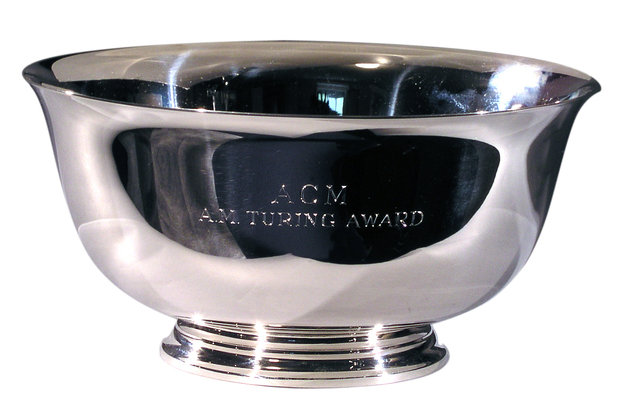
\includegraphics[scale=0.65]{turing_bowl.jpg}
 \caption{A.M. TURING AWARD}
\end{figure}
\newpage

\tableofcontents

\begin{figure}[!htb]
 \centering
 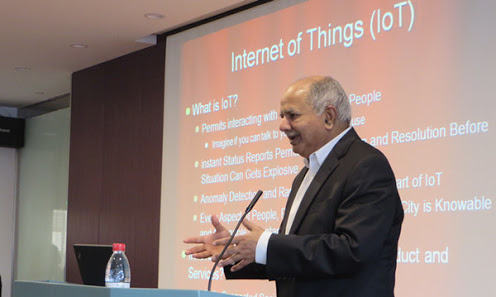
\includegraphics[scale=0.75]{raj1.jpg}
 \caption{Raj reddy first indian turing award winner}
\end{figure}


\newpage
  
%\begin{abstract}
\section{Introduction}

\begin{wrapfigure}{l}{7cm}
 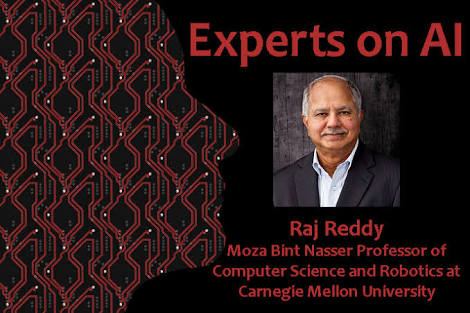
\includegraphics[scale=0.4]{raj.jpg}
 \caption{Raj Reddy}
\end{wrapfigure}

  \textbf{Dabbala Rajagopal ``Raj'' Reddy \cite{1}} 
  is an indian-american computer 
  Scientist and a winner of Turing award. He is one of the early 
  pioneers of Artificial Intelligence and has saerved on the faculty 
  of Stanford and carnegie mellon university for over 40 years. He 
  was the founding director of Robotics Insitute at carnegie mellon university.
  He was instumental in helping to create {\bf Rajiv Gandhi University of 
  KnowledgeTechnologies} in india,to cater to the educational needs of 
  low-income,gifted,rural youth. He is also the chairman of 
  {\bf Internatinal Insitute of Information Technologies,Hyderabad.}
  He is the first person of Asian origin to recieve {\bf ACM Turing Award}, in 
  1994,the highest award in Computer science,for his work in the field of 
  Artificial Intelligence.
  
  
\section{Early Life}  
  Dabbala Rajagopal Reddy was born in katur,chitoor district,Madras Presidency,
  British Raj.His father, Sreenivasulu Reddy, was an agricultural landlord,and 
  his mother,Pitchamma was a  homemaker.                   
  
\begin{table}[!hbt]
 \centering
 \caption{\bf Qualification}
  \begin{tabular}{|c|c|c|c|}
    \hline
    {\bf Degree} & {\bf Specilization} & {\bf Year} & {\bf Institute}\\
    \hline
    Bachelor of science & civil engneering & 1958 & 
    \begin{minipage}{0.295\textwidth} 
      University of Madras(now {\bf Anna University})
    \end{minipage}\\
    \hline
    Master of science & Information Technology & 1960 & University of new south wales\\
    \hline
    Doctrate & Computer science & 1966 & Stanford university\\
    \hline
  \end{tabular}
\end{table}

\section{Career}
\paragraph{}
  Reddy is the Moza Bint Nasser University Professor of Computer Science and
  Robotics in the school of computer science at Carnegie Mellon University.
  From 1960,Reddy worked for IBM in Australia.He was an Assistant Professor
  of Computer Science at Stanford university from 1966 to 1969.He joined 
  the Carnegie Mellon faculty as an associate professor of Computer Science in
  1969. He became a full professor in 1973 and a university professor, in 1984.
  He was the founding director of the Robotics Institute from 1979 to 1991 
  and the Dean of School of Computer Science from 1991 to 1999. As a dean of 
  SCS, he helped create the Language Technologies Institute, Human Computer 
  Interaction Institute, Center for Automated Learning and Discovery (since 
  renamed as the Machine Learning Department), and the Institute for Software
  Research. He is the chairman of Governing Council of IIIT Hyderabad and he 
  is the Chancellor and the chairman of the Governing Council of the Rajiv 
  Gandhi University of Knowledge Technologies, India.
  
  Reddy was a co-chair of the President's Information Technology Advisory 
  Committee (PITAC) from 1999 to 2001. He was one of the founders of the 
  American Association for Artificial Intelligence and was its President
  from 1987 to 1989.He serves on the International board of governors of 
  Peres Center for Peace in Israel.He served as a member of the governing 
  councils of EMRI and HMRI which use technology-enabled solutions to provide
  cost-effective health care coverage to rural population in India.
  
\section{Research}
\paragraph{}
  Reddy's early research was conducted at the AI labs at Stanford, first as 
  a graduate student and later as an Assistant Professor, and at CMU since 1969.
  His AI research concentrated on perceptual and motor aspect of intelligence 
  such as speech, language, vision and robotics.Over a span of three decades, 
  Reddy and his colleagues created several historic demonstrations of spoken 
  language systems, e.g., voice control of a robot, large vocabulary connected
  speech recognition, speaker independent speech recognition, and unrestricted 
  vocabulary dictation.Reddy and his colleagues have also made seminal 
  contributions to Task Oriented Computer Architectures, Analysis of Natural 
  Scenes, Universal Access to Information,and Autonomous Robotic Systems.
  Hearsay I was one of the first systems capable of continuous speech 
  recognition.Subsequent systems like Hearsay II, Dragon, Harpy, and 
  Sphinx I/II developed many of the ideas underlying modern commercial speech 
  recognition technology as summarized in his recent historical review of 
  speech recognition with Xuedong Huang and James K. Baker.Some of these 
  ideas—most notably the "blackboard model" for coordinating multiple knowledge
  sources—have been adopted across the spectrum of applied artificial 
  intelligence.His other major research interest has been in exploring the 
  role of "Technology in Service of Society".An early attempt in this area 
  was the establishment, in 1981, of the fr: Centre Mondial Informatique et 
  Ressource Humaine in France by Jean-Jacques Servan-Schreiber and a 
  technical team of Nicholas Negroponte, Alan Kay, Seymour Papert and 
  Terry Winograd.Reddy served as the Chief Scientist for the center.
  
  Since 1995, Reddy and colleagues in China and India have worked on 
  "Universal Digital Library Project".The project is currently attempting 
  to archive 1,000 newspapers for the next 1,000 years and provide online 
  access to UNESCO heritage sites.His current research centers around 
  “Technology in Service of Society”, in particular creating voice only 
  dialog based Apps for tasks such as online shopping and banking, online
  voting, a reading app that would read newspapers to people who cannot 
  read, and dynamic realtime speech-to-speech translation of TV shows and 
  lectures into local languages; all to enable semi-literate people in rural
  communities with connectivity and smart phones to benefit from advances in
  technology.
  
  
   
\section{Awards and Honors}
   
\begin{figure}[!htb]
  \centering
  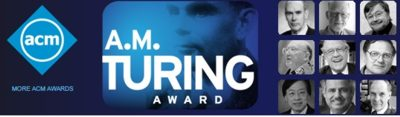
\includegraphics[scale=0.5]{turing.jpg}
  \caption{ACM Turing Award}
\end{figure}
    

   
\begin{table}[!htb]
%\begin{minipage}{\textwidth}
  \centering
  \caption{\bf Awards}
  \begin{tabular}{||c|c|c||}
  \hline
  {\bf Award} & {\bf Year } & {\bf Organisation}\\
  \hline
  French Legion of Honor & 1984 & French President\\
  Turing Award & 1994 & ACM\footnotemark\\
  Padma bhushan & 2001 & Indian Government\\
  Vannevar Bush Award & 2006 & US government\\
  \hline
  \end{tabular}
%\end{minipage}
\end{table}
\footnotetext{Association for Computer Machinery}
    
\begin{figure}[!hbt]
  \centering
  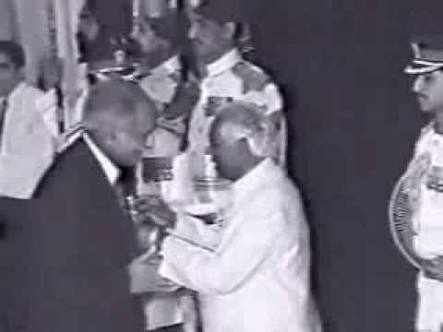
\includegraphics[scale=0.5]{pb.jpg}
  \caption{Raj reddy reciving padma bhushan}
\end{figure}
  
%   \newpage
\begin{figure}[!hbt]
  \centering
  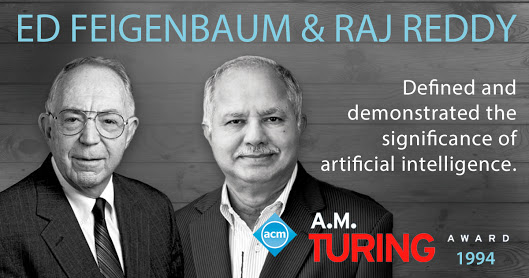
\includegraphics[scale=0.8]{rajco.jpg}
  \caption{Raj reddy and ED Feignbaum}
\end{figure}

\section{Contributions}
 \begin{enumerate}
  \item[6.1] Machine Intelligence and Robotics: Report of the NASA Study Group —
  Executive Summary, Final Report Carl Sagan (chair), Raj Reddy (vice chair) 
  and others, NASA JPL, September 1979.
  \item[6.2] Foundations and Grand Challenges of Artificial Intelligence, AAAI 
  Presidential Address, 1988.
  \item[6.3] To Dream the Possible Dream, Turing Award Lecture presented at ACM 
  CS Conference, March 1, 1995 
 \end{enumerate}

\begin{thebibliography}{10}
\bibitem{1}
 https://en.wikipedia.org/wiki/Raj Reddy
\end{thebibliography}



\end{document}
